\documentclass{article}

% Language setting
% Replace `english' with e.g. `spanish' to change the document language
\usepackage[english]{babel}

% Set page size and margins
% Replace `letterpaper' with`a4paper' for UK/EU standard size
\usepackage[letterpaper,top=2cm,bottom=2cm,left=3cm,right=3cm,marginparwidth=1.75cm]{geometry}
\usepackage{float}
% Useful packages
\usepackage{amsmath}
\usepackage{graphicx}
\usepackage[colorlinks=true, allcolors=blue]{hyperref}
\usepackage{fancyvrb}
\usepackage{fontspec}
\usepackage{parskip}
\usepackage[dvipsnames]{xcolor}
\usepackage{xparse}
\usepackage{listings}
\definecolor{codegrey}{rgb}{0.8,0.8,0.8}
\lstset{
    basicstyle=\ttfamily,
    breaklines=true,
    backgroundcolor=\color{codegrey}
}
\usepackage{realboxes}
\newcommand{\code}[1]{\colorbox{codegrey}{\lstinline|#1|}}

\setmainfont{Arial}

\linespread{1.2}

\title{Visual Studio Code Setup Guide}



\VerbatimFootnotes
\begin{document}
\centering
\Large Visual Studio Code Setup Guide\par
\large EEEN30222 Computer Systems Architecture

\normalsize\raggedright
\section{Prerequisites}

If you are working on a University Computer, skip to Section \ref{Section_3}.


This guide is a simplified version of Microsoft's own \href{https://code.visualstudio.com/docs/cpp/config-mingw}{setup guide for C++}, with a few elements changed to reflect the needs of this course. 
Before setting up Visual Visual Studio Code (VSC), you will need a C compiler. The recommended compiler is gcc, which is already installed on the university systems via mingw. To install it on your own system, visit \href{https://www.mingw-w64.org/}{the mingw site}. The full installation process is documented in \href{https://www.youtube.com/watch?v=oC69vlWofJQ}{this video}. To install mingw on an Apple device, \href{https://www.macports.org/install.php}{install MacPorts} and then run \code{sudo port install mingw-w64}. Although they will try to help, it is not possible for the Lab Demonstrators to learn the details of every possible OS and computer setup. We ask you to try and use the University computers if you are having trouble with your own system. 

\section{Installing VSC and Extensions}
First, \href{https://code.visualstudio.com/download}{download} VSC. Take care not to download Visual Studio, as that is a separate program that we do not need. The installer can be run with the default settings. Once the installation is complete, you will likely be greeted with some release notes. You can close these, and the welcome screen. \par
VSC has a wide array of extensions available to enable operation in many languages and platforms. Since this course uses the C programming language, the associated extensions may prove useful. 
Go to the extensions tab on the left and install the C/C++ extension by Microsoft. You may also wish to install other extensions. There are a variety of tools to assist with git integration, and several AI code assistants available.
\begin{figure}[h]
    \centering
    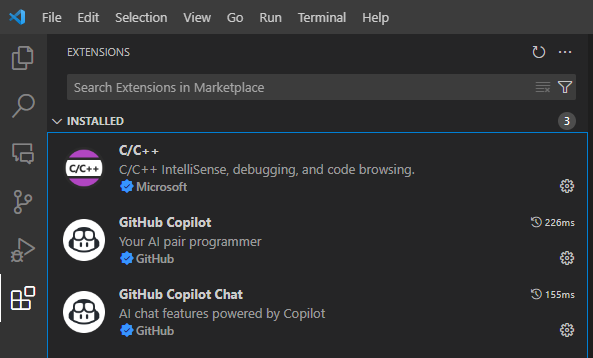
\includegraphics[width=0.5\linewidth]{extensions.png}
    \label{fig:enter-label}
\end{figure}

\section{Creating and configuring the project}\label{Section_3}

VSC operates using a workspace which is simply an open folder on the PC. Go to the explorer tab on the left, and select \code{Open Folder}. This will open file explorer, where you can choose the location that your files will be saved. 
\par
\textbf{NOTE: } If you are on a university PC, navigate to \code{This PC > home\$(\\nask.man.ac.uk)(P:)} and put your folder there\footnote{If you navigate this way, VSC sets the directory to \code{P:\\...}, whereas other navigation approaches set it to \code{\\\\nask.man.ac.uk\\home\$\\...} which causes errors.}. 
\par 
Create a blank folder with any name, and open it. You may have to indicate that you trust this folder. Since you created it, and it is empty, it can be trusted. Now, in VSC, right click in the explorer panel to create a new file, and call it \code{main.c}. VSC will automatically recognise it as a C file, and highlight keywords to make the code easier to read. Your explorer should now look like this:
\begin{figure}[H]
    \centering
    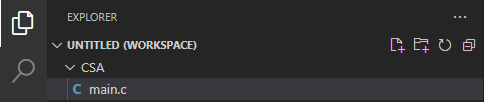
\includegraphics[width=0.5\linewidth]{explorer.png}
    \label{fig:enter-label}
\end{figure}

Copy the following code into \code{main.c} and save the file:

\begin{verbatim}
#include <stdio.h> 
int main() {
   printf("Hello, World!");
   return 0;
}
\end{verbatim}

Now, the file needs compiling. When using compile or run commands, they are applied to the active file, so select \code{main.c}. Then, go to \code{Terminal > Run Build Task} or press Ctrl + Shift + B. If mingw was installed correctly, the following dialogue should appear as VSC finds the correct compiler.

\begin{figure}[h]
    \centering
    \includegraphics[width=0.5\linewidth]{Compiler.png}
    \label{fig:enter-label}
\end{figure}

Don't worry if there are multiple options, it just means that VSC has found multiple C++ compilers. Select \code{C/C++: gcc.exe build active file}. In the Terminal, you will see the build command running and the build outputs. In your file explorer, if the build was successful, you should see a file called main.exe. If you type \code{./main.exe} into the terminal, you should see the output \code{Hello, World!}
\begin{figure}[h]
    \centering
    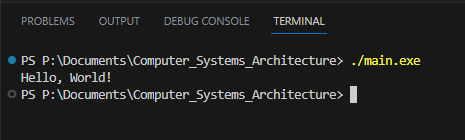
\includegraphics[width=0.5\linewidth]{output.png}
    \label{fig:enter-label}
\end{figure}
\newpage
\section{Debugging}
If you wish, this is enough to be getting on with. However, manually compiling and typing \code{./main.exe} can get a bit tiresome. VSC enables compiling, running, and debugging a file with one button. Go to  \code{Terminal > Configure Default Build Task}. In the same dialogue as before, select \code{C/C++: gcc.exe build active file}. This creates a new folder and file, \code{/.vscode/tasks.json}. In there are the configuration parameters to build the file. Now, typing Ctrl + Shift + B will attempt to compile the active file. Try it with \code{main.c} open. The compilation will fail if you have \code{tasks.json} selected, as this is not a C file.
\par
For running and debugging, go to the Run and Debug tab on the left. With \code{main.c} open, select \code{create a launch.json file}, then in the dialogue that appears, select \code{C++ (GDB/LLDB)}. This will again create a new config file, but this time we need to edit it. Paste the code on the next page into your \code{launch.json}.
\par
The key changes from the default \code{launch.json} are: the program name has been set, the debugger path removed such that VSC will find it automatically, and a pre-launch task has been added, linked to the build task we set up earlier. This means that, when you run your code, VSC will compile it automatically first. Now, go to the \code{Run and Debug} tab on the left, and click the green run icon at the top (the drop-down should say \code{(gdb) Launch}). Alternatively, press F5. At the bottom of the screen, the debug console contains information about the process, and the program output is in the terminal as before. You can now add breakpoints to your code (by clicking next to the line numbers), and the debugger will stop at the break point. The controls at the top can then be used to step through your code one line at a time, and you can watch the values of your variables in the left panel. 
\par
Pay attention to the \code{args} line in the \code{launch.json} file. The coursework requires you to make use of command line arguments, and if you are running your file using this setup, your command line arguments must go on that line in \code{launch.json}.

\newpage
\subsection{launch.json configuration parameters.}
\begin{verbatim}
{
"configurations": [
    {   
        "preLaunchTask": "C/C++: gcc.exe build active file",
        "name": "(gdb) Launch",
        "type": "cppdbg",
        "request": "launch",
        "program": "${fileDirname}\\${fileBasenameNoExtension}.exe",
        "args": [],
        "stopAtEntry": false,
        "cwd": "${fileDirname}",
        "environment": [],
        "externalConsole": false,
        "MIMode": "gdb",
        "setupCommands": [
            {
                "description": "Enable pretty-printing for gdb",
                "text": "-enable-pretty-printing",
                "ignoreFailures": true
            },
            {
                "description": "Set Disassembly Flavor to Intel",
                "text": "-gdb-set disassembly-flavor intel",
                "ignoreFailures": true
            }
        ]
    }
]
}
\end{verbatim}

\par
26/02/24\par
Christopher Blum\par
This document was created in Latex, the source code is available \href{https://github.com/PrimaryComet/CSA-VSCode-Setup-Guide}{on Github}.
\end{document}